% Generated by pysimcount.figratio -- do not edit; regenerate instead.
% figure: main-cnot-all-formulas -- cost ratio to Blanes \& Moan q=10 vs n, one panel per family
% seeds [1, 2, 3, 4, 5, 6, 7, 8, 9, 10]; metric=cnot kind=xyz merged (cz, simcount template)
% shown: suzuki4, suzuki6, mo-q6, mo-q14, bm-q10, mo-o8-q21, morales-y8m10, morales-m8
% removed (see main-cnot-all-formulas-ranking.md): lie-trotter, suzuki2, suzuki8
% y = paired ratio to bm-q10: geometric mean over seeds of each seed's ratio; bars min..max over seeds
% extrapolated n: each seed's own power-law fit, r = ceil(a_s n^b_s); per-step counts exact
% bars of the absolute figure are not these bars: the same seed is used in both formulas
% single-axis ratio figure draws bars only at n = [4, 5, 6, 7, 8, 10, 30, 100, 500]; the panel figure draws all
% derived: main-cnot-all-formulas.json by pysimcount.figratio; source_sha256=500e44d2dcd8af1b87c0e674b1bbfda8db5fe55c084698bcdf0ad96a67f293ce
% figure made at git_commit=e5d9ee696f892e28aced765585653760f8a427c4 git_dirty=False
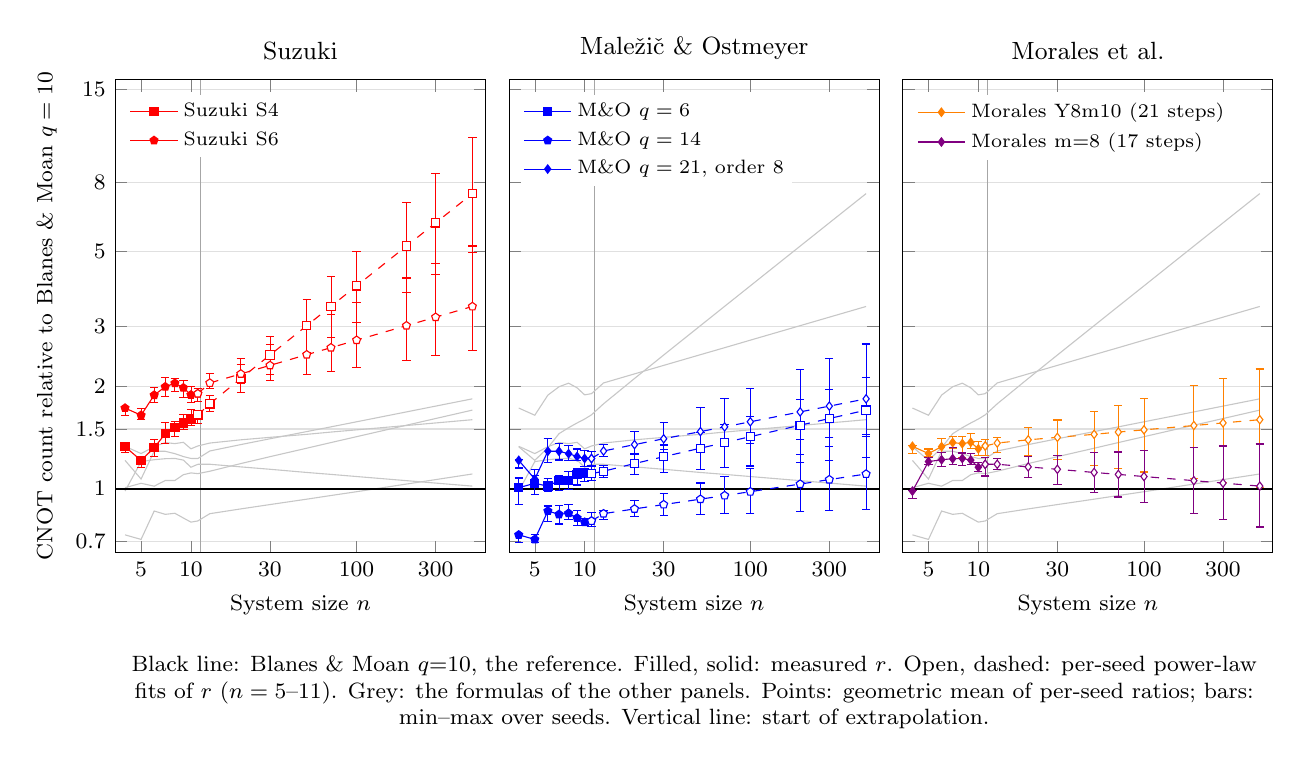
\begin{tikzpicture}
  \begin{loglogaxis}[
    scale only axis,
    at={(0.0cm,0.0cm)}, anchor=south west,
    width=4.7cm, height=6.0cm,
    title={Suzuki}, title style={font=\small, yshift=-2pt},
    xtick={5,10,30,100,300}, xticklabels={5,10,30,100,300},
    tick label style={font=\footnotesize},
    xmin=3.5, xmax=600, ymin=0.65, ymax=16,
    ymajorgrids=true, grid style={black!12},
    legend pos=north west,
    legend style={draw=none, fill=white, font=\scriptsize, inner sep=1pt},
    legend cell align=left,
    ytick={0.7,1,1.5,2,3,5,8,15}, yticklabels={0.7,1,1.5,2,3,5,8,15}, yminorticks=false,
    xlabel={System size $n$}, xlabel style={font=\footnotesize},
    ylabel={CNOT count relative to Blanes \& Moan $q=10$}, ylabel style={font=\footnotesize},
  ]
    \draw[black!35] (axis cs:11.4,0.65) -- (axis cs:11.4,16);
    \addplot[black!22, solid, no markers, forget plot] coordinates {
      (4,1.00745)
      (5,1.03803)
      (6,1.01776)
      (7,1.05796)
      (8,1.05779)
      (9,1.10025)
      (10,1.11364)
      (11,1.10823)
      (13,1.12639)
      (20,1.18647)
      (30,1.24318)
      (50,1.31671)
      (70,1.368)
      (100,1.42391)
      (200,1.53886)
      (300,1.61027)
      (500,1.70505)
    };
    \addplot[black!22, solid, no markers, forget plot] coordinates {
      (4,0.731817)
      (5,0.709531)
      (6,0.860092)
      (7,0.84085)
      (8,0.846993)
      (9,0.820349)
      (10,0.797771)
      (11,0.804072)
      (13,0.844688)
      (20,0.872506)
      (30,0.898554)
      (50,0.931988)
      (70,0.955429)
      (100,0.980414)
      (200,1.03266)
      (300,1.06423)
      (500,1.10559)
    };
    \addplot[black!22, solid, no markers, forget plot] coordinates {
      (4,1.21256)
      (5,1.06821)
      (6,1.29039)
      (7,1.28945)
      (8,1.26895)
      (9,1.24433)
      (10,1.22847)
      (11,1.22744)
      (13,1.2921)
      (20,1.34936)
      (30,1.40374)
      (50,1.47376)
      (70,1.52175)
      (100,1.57507)
      (200,1.68418)
      (300,1.75166)
      (500,1.84036)
    };
    \addplot[black!22, solid, no markers, forget plot] coordinates {
      (4,1.33382)
      (5,1.26969)
      (6,1.33063)
      (7,1.36813)
      (8,1.35846)
      (9,1.37031)
      (10,1.31126)
      (11,1.33672)
      (13,1.3636)
      (20,1.39375)
      (30,1.41739)
      (50,1.44666)
      (70,1.46912)
      (100,1.49133)
      (200,1.53574)
      (300,1.56277)
      (500,1.59764)
    };
    \addplot[black!22, solid, no markers, forget plot] coordinates {
      (4,0.984315)
      (5,1.20247)
      (6,1.21776)
      (7,1.22634)
      (8,1.22852)
      (9,1.21473)
      (10,1.15733)
      (11,1.18055)
      (13,1.18101)
      (20,1.16004)
      (30,1.14149)
      (50,1.11703)
      (70,1.10256)
      (100,1.08665)
      (200,1.05674)
      (300,1.0394)
      (500,1.01832)
    };
    \addplot[black, solid, line width=0.9pt, no markers, forget plot] coordinates {(3.5,1) (600,1)};
    \addplot[red, solid, mark=square*, mark size=1.5pt, mark options={solid, fill=red}, error bars/.cd, y dir=both, y explicit, error bar style={solid, line width=0.3pt}] coordinates {
      (4,1.33003) += (0,0.0257827) -= (0,0.0495402)
      (5,1.21263) += (0,0.0274181) -= (0,0.0601942)
      (6,1.32096) += (0,0.0777238) -= (0,0.0798747)
      (7,1.45283) += (0,0.119082) -= (0,0.0928605)
      (8,1.51334) += (0,0.0684355) -= (0,0.0875031)
      (9,1.56253) += (0,0.0922568) -= (0,0.0634198)
      (10,1.60481) += (0,0.102509) -= (0,0.0682229)
      (11,1.65113) += (0,0.0422449) -= (0,0.0952214)
    };
    \addlegendentry{Suzuki S4}
    \addplot[red, dashed, mark=square*, mark size=1.5pt, mark options={solid, fill=white}, forget plot, error bars/.cd, y dir=both, y explicit, error bar style={solid, line width=0.3pt}] coordinates {
      (11,1.65113)
      (13,1.77927) += (0,0.0987811) -= (0,0.0929638)
      (20,2.11227) += (0,0.217231) -= (0,0.192694)
      (30,2.47662) += (0,0.338937) -= (0,0.310927)
      (50,3.02271) += (0,0.577528) -= (0,0.501472)
      (70,3.44606) += (0,0.779828) -= (0,0.661843)
      (100,3.95946) += (0,1.0518) -= (0,0.870848)
      (200,5.18403) += (0,1.79622) -= (0,1.39783)
      (300,6.06858) += (0,2.40101) -= (0,1.8031)
      (500,7.40094) += (0,3.40301) -= (0,2.44585)
    };
    \addplot[red, solid, mark=pentagon*, mark size=1.5pt, mark options={solid, fill=red}, error bars/.cd, y dir=both, y explicit, error bar style={solid, line width=0.3pt}] coordinates {
      (4,1.72897) += (0,0.00991082) -= (0,0.0866937)
      (5,1.64657) += (0,0.0778214) -= (0,0.0453494)
      (6,1.88761) += (0,0.10207) -= (0,0.0874236)
      (7,1.99748) += (0,0.126153) -= (0,0.128683)
      (8,2.04638) += (0,0.0651142) -= (0,0.1156)
      (9,1.98351) += (0,0.100916) -= (0,0.12093)
      (10,1.89091) += (0,0.110618) -= (0,0.0946666)
      (11,1.90609) += (0,0.0646381) -= (0,0.0933922)
    };
    \addlegendentry{Suzuki S6}
    \addplot[red, dashed, mark=pentagon*, mark size=1.5pt, mark options={solid, fill=white}, forget plot, error bars/.cd, y dir=both, y explicit, error bar style={solid, line width=0.3pt}] coordinates {
      (11,1.90609)
      (13,2.04943) += (0,0.140274) -= (0,0.078696)
      (20,2.17945) += (0,0.236589) -= (0,0.137703)
      (30,2.30877) += (0,0.344139) -= (0,0.220222)
      (50,2.48268) += (0,0.521101) -= (0,0.30949)
      (70,2.60322) += (0,0.647635) -= (0,0.3815)
      (100,2.73936) += (0,0.799193) -= (0,0.460178)
      (200,3.0225) += (0,1.1528) -= (0,0.628971)
      (300,3.20167) += (0,1.39514) -= (0,0.737505)
      (500,3.44277) += (0,1.74589) -= (0,0.887415)
    };
  \end{loglogaxis}
  \begin{loglogaxis}[
    scale only axis,
    at={(5.0cm,0.0cm)}, anchor=south west,
    width=4.7cm, height=6.0cm,
    title={Male\v{z}i\v{c} \& Ostmeyer}, title style={font=\small, yshift=-2pt},
    xtick={5,10,30,100,300}, xticklabels={5,10,30,100,300},
    tick label style={font=\footnotesize},
    xmin=3.5, xmax=600, ymin=0.65, ymax=16,
    ymajorgrids=true, grid style={black!12},
    legend pos=north west,
    legend style={draw=none, fill=white, font=\scriptsize, inner sep=1pt},
    legend cell align=left,
    ytick={0.7,1,1.5,2,3,5,8,15}, yticklabels={0.7,1,1.5,2,3,5,8,15}, yminorticks=false,
    xlabel={System size $n$}, xlabel style={font=\footnotesize},
    yticklabels={},
  ]
    \draw[black!35] (axis cs:11.4,0.65) -- (axis cs:11.4,16);
    \addplot[black!22, solid, no markers, forget plot] coordinates {
      (4,1.33003)
      (5,1.21263)
      (6,1.32096)
      (7,1.45283)
      (8,1.51334)
      (9,1.56253)
      (10,1.60481)
      (11,1.65113)
      (13,1.77927)
      (20,2.11227)
      (30,2.47662)
      (50,3.02271)
      (70,3.44606)
      (100,3.95946)
      (200,5.18403)
      (300,6.06858)
      (500,7.40094)
    };
    \addplot[black!22, solid, no markers, forget plot] coordinates {
      (4,1.72897)
      (5,1.64657)
      (6,1.88761)
      (7,1.99748)
      (8,2.04638)
      (9,1.98351)
      (10,1.89091)
      (11,1.90609)
      (13,2.04943)
      (20,2.17945)
      (30,2.30877)
      (50,2.48268)
      (70,2.60322)
      (100,2.73936)
      (200,3.0225)
      (300,3.20167)
      (500,3.44277)
    };
    \addplot[black!22, solid, no markers, forget plot] coordinates {
      (4,1.33382)
      (5,1.26969)
      (6,1.33063)
      (7,1.36813)
      (8,1.35846)
      (9,1.37031)
      (10,1.31126)
      (11,1.33672)
      (13,1.3636)
      (20,1.39375)
      (30,1.41739)
      (50,1.44666)
      (70,1.46912)
      (100,1.49133)
      (200,1.53574)
      (300,1.56277)
      (500,1.59764)
    };
    \addplot[black!22, solid, no markers, forget plot] coordinates {
      (4,0.984315)
      (5,1.20247)
      (6,1.21776)
      (7,1.22634)
      (8,1.22852)
      (9,1.21473)
      (10,1.15733)
      (11,1.18055)
      (13,1.18101)
      (20,1.16004)
      (30,1.14149)
      (50,1.11703)
      (70,1.10256)
      (100,1.08665)
      (200,1.05674)
      (300,1.0394)
      (500,1.01832)
    };
    \addplot[black, solid, line width=0.9pt, no markers, forget plot] coordinates {(3.5,1) (600,1)};
    \addplot[blue, solid, mark=square*, mark size=1.5pt, mark options={solid, fill=blue}, error bars/.cd, y dir=both, y explicit, error bar style={solid, line width=0.3pt}] coordinates {
      (4,1.00745) += (0,0.0685886) -= (0,0.110751)
      (5,1.03803) += (0,0.0531075) -= (0,0.0752622)
      (6,1.01776) += (0,0.0554134) -= (0,0.0327667)
      (7,1.05796) += (0,0.0353953) -= (0,0.0697351)
      (8,1.05779) += (0,0.0693399) -= (0,0.0647537)
      (9,1.10025) += (0,0.0430411) -= (0,0.0740767)
      (10,1.11364) += (0,0.029656) -= (0,0.0627804)
      (11,1.10823) += (0,0.0548253) -= (0,0.0504878)
    };
    \addlegendentry{M\&O $q=6$}
    \addplot[blue, dashed, mark=square*, mark size=1.5pt, mark options={solid, fill=white}, forget plot, error bars/.cd, y dir=both, y explicit, error bar style={solid, line width=0.3pt}] coordinates {
      (11,1.10823)
      (13,1.12639) += (0,0.0462218) -= (0,0.0475869)
      (20,1.18647) += (0,0.0714966) -= (0,0.0823157)
      (30,1.24318) += (0,0.102945) -= (0,0.123088)
      (50,1.31671) += (0,0.144938) -= (0,0.176045)
      (70,1.368) += (0,0.176794) -= (0,0.214064)
      (100,1.42391) += (0,0.212846) -= (0,0.256618)
      (200,1.53886) += (0,0.293578) -= (0,0.342828)
      (300,1.61027) += (0,0.346669) -= (0,0.397082)
      (500,1.70505) += (0,0.421195) -= (0,0.47014)
    };
    \addplot[blue, solid, mark=pentagon*, mark size=1.5pt, mark options={solid, fill=blue}, error bars/.cd, y dir=both, y explicit, error bar style={solid, line width=0.3pt}] coordinates {
      (4,0.731817) += (0,0.00419492) -= (0,0.0366946)
      (5,0.709531) += (0,0.022176) -= (0,0.0144094)
      (6,0.860092) += (0,0.0296644) -= (0,0.0580279)
      (7,0.84085) += (0,0.0528778) -= (0,0.0530456)
      (8,0.846993) += (0,0.0525769) -= (0,0.0360171)
      (9,0.820349) += (0,0.0438564) -= (0,0.0404563)
      (10,0.797771) += (0,0.018242) -= (0,0.0157585)
      (11,0.804072) += (0,0.0470977) -= (0,0.0317143)
    };
    \addlegendentry{M\&O $q=14$}
    \addplot[blue, dashed, mark=pentagon*, mark size=1.5pt, mark options={solid, fill=white}, forget plot, error bars/.cd, y dir=both, y explicit, error bar style={solid, line width=0.3pt}] coordinates {
      (11,0.804072)
      (13,0.844688) += (0,0.0159388) -= (0,0.0319304)
      (20,0.872506) += (0,0.0498677) -= (0,0.0458742)
      (30,0.898554) += (0,0.0721487) -= (0,0.0644078)
      (50,0.931988) += (0,0.108452) -= (0,0.093116)
      (70,0.955429) += (0,0.134546) -= (0,0.111997)
      (100,0.980414) += (0,0.164377) -= (0,0.134107)
      (200,1.03266) += (0,0.226814) -= (0,0.177445)
      (300,1.06423) += (0,0.267643) -= (0,0.203272)
      (500,1.10559) += (0,0.322462) -= (0,0.238031)
    };
    \addplot[blue, solid, mark=diamond*, mark size=1.5pt, mark options={solid, fill=blue}, error bars/.cd, y dir=both, y explicit, error bar style={solid, line width=0.3pt}] coordinates {
      (4,1.21256) += (0,0.00695065) -= (0,0.0608)
      (5,1.06821) += (0,0.0720382) -= (0,0.0316204)
      (6,1.29039) += (0,0.119364) -= (0,0.0943322)
      (7,1.28945) += (0,0.0688295) -= (0,0.0741478)
      (8,1.26895) += (0,0.0725147) -= (0,0.0595991)
      (9,1.24433) += (0,0.0650391) -= (0,0.0307685)
      (10,1.22847) += (0,0.0672644) -= (0,0.0623087)
      (11,1.22744) += (0,0.0579253) -= (0,0.0539477)
    };
    \addlegendentry{M\&O $q=21$, order 8}
    \addplot[blue, dashed, mark=diamond*, mark size=1.5pt, mark options={solid, fill=white}, forget plot, error bars/.cd, y dir=both, y explicit, error bar style={solid, line width=0.3pt}] coordinates {
      (11,1.22744)
      (13,1.2921) += (0,0.0571112) -= (0,0.0481927)
      (20,1.34936) += (0,0.12578) -= (0,0.0793106)
      (30,1.40374) += (0,0.166468) -= (0,0.100932)
      (50,1.47376) += (0,0.258342) -= (0,0.151736)
      (70,1.52175) += (0,0.323063) -= (0,0.177951)
      (100,1.57507) += (0,0.398539) -= (0,0.214632)
      (200,1.68418) += (0,0.563468) -= (0,0.28736)
      (300,1.75166) += (0,0.673631) -= (0,0.33351)
      (500,1.84036) += (0,0.828468) -= (0,0.394541)
    };
  \end{loglogaxis}
  \begin{loglogaxis}[
    scale only axis,
    at={(10.0cm,0.0cm)}, anchor=south west,
    width=4.7cm, height=6.0cm,
    title={Morales et al.}, title style={font=\small, yshift=-2pt},
    xtick={5,10,30,100,300}, xticklabels={5,10,30,100,300},
    tick label style={font=\footnotesize},
    xmin=3.5, xmax=600, ymin=0.65, ymax=16,
    ymajorgrids=true, grid style={black!12},
    legend pos=north west,
    legend style={draw=none, fill=white, font=\scriptsize, inner sep=1pt},
    legend cell align=left,
    ytick={0.7,1,1.5,2,3,5,8,15}, yticklabels={0.7,1,1.5,2,3,5,8,15}, yminorticks=false,
    xlabel={System size $n$}, xlabel style={font=\footnotesize},
    yticklabels={},
  ]
    \draw[black!35] (axis cs:11.4,0.65) -- (axis cs:11.4,16);
    \addplot[black!22, solid, no markers, forget plot] coordinates {
      (4,1.33003)
      (5,1.21263)
      (6,1.32096)
      (7,1.45283)
      (8,1.51334)
      (9,1.56253)
      (10,1.60481)
      (11,1.65113)
      (13,1.77927)
      (20,2.11227)
      (30,2.47662)
      (50,3.02271)
      (70,3.44606)
      (100,3.95946)
      (200,5.18403)
      (300,6.06858)
      (500,7.40094)
    };
    \addplot[black!22, solid, no markers, forget plot] coordinates {
      (4,1.72897)
      (5,1.64657)
      (6,1.88761)
      (7,1.99748)
      (8,2.04638)
      (9,1.98351)
      (10,1.89091)
      (11,1.90609)
      (13,2.04943)
      (20,2.17945)
      (30,2.30877)
      (50,2.48268)
      (70,2.60322)
      (100,2.73936)
      (200,3.0225)
      (300,3.20167)
      (500,3.44277)
    };
    \addplot[black!22, solid, no markers, forget plot] coordinates {
      (4,1.00745)
      (5,1.03803)
      (6,1.01776)
      (7,1.05796)
      (8,1.05779)
      (9,1.10025)
      (10,1.11364)
      (11,1.10823)
      (13,1.12639)
      (20,1.18647)
      (30,1.24318)
      (50,1.31671)
      (70,1.368)
      (100,1.42391)
      (200,1.53886)
      (300,1.61027)
      (500,1.70505)
    };
    \addplot[black!22, solid, no markers, forget plot] coordinates {
      (4,0.731817)
      (5,0.709531)
      (6,0.860092)
      (7,0.84085)
      (8,0.846993)
      (9,0.820349)
      (10,0.797771)
      (11,0.804072)
      (13,0.844688)
      (20,0.872506)
      (30,0.898554)
      (50,0.931988)
      (70,0.955429)
      (100,0.980414)
      (200,1.03266)
      (300,1.06423)
      (500,1.10559)
    };
    \addplot[black!22, solid, no markers, forget plot] coordinates {
      (4,1.21256)
      (5,1.06821)
      (6,1.29039)
      (7,1.28945)
      (8,1.26895)
      (9,1.24433)
      (10,1.22847)
      (11,1.22744)
      (13,1.2921)
      (20,1.34936)
      (30,1.40374)
      (50,1.47376)
      (70,1.52175)
      (100,1.57507)
      (200,1.68418)
      (300,1.75166)
      (500,1.84036)
    };
    \addplot[black, solid, line width=0.9pt, no markers, forget plot] coordinates {(3.5,1) (600,1)};
    \addplot[orange, solid, mark=diamond*, mark size=1.5pt, mark options={solid, fill=orange}, error bars/.cd, y dir=both, y explicit, error bar style={solid, line width=0.3pt}] coordinates {
      (4,1.33382) += (0,0.00764572) -= (0,0.06688)
      (5,1.26969) += (0,0.0396834) -= (0,0.0257852)
      (6,1.33063) += (0,0.0791296) -= (0,0.0548291)
      (7,1.36813) += (0,0.0616389) -= (0,0.0551259)
      (8,1.35846) += (0,0.0631424) -= (0,0.125764)
      (9,1.37031) += (0,0.086515) -= (0,0.0556141)
      (10,1.31126) += (0,0.0708534) -= (0,0.0587197)
      (11,1.33672) += (0,0.0594946) -= (0,0.0849967)
    };
    \addlegendentry{Morales Y8m10 (21 steps)}
    \addplot[orange, dashed, mark=diamond*, mark size=1.5pt, mark options={solid, fill=white}, forget plot, error bars/.cd, y dir=both, y explicit, error bar style={solid, line width=0.3pt}] coordinates {
      (11,1.33672)
      (13,1.3636) += (0,0.0514183) -= (0,0.0878056)
      (20,1.39375) += (0,0.121262) -= (0,0.142374)
      (30,1.41739) += (0,0.177353) -= (0,0.200533)
      (50,1.44666) += (0,0.245316) -= (0,0.273053)
      (70,1.46912) += (0,0.295088) -= (0,0.319099)
      (100,1.49133) += (0,0.353436) -= (0,0.370972)
      (200,1.53574) += (0,0.475847) -= (0,0.465551)
      (300,1.56277) += (0,0.552336) -= (0,0.520813)
      (500,1.59764) += (0,0.655004) -= (0,0.590736)
    };
    \addplot[violet, solid, mark=diamond*, mark size=1.5pt, mark options={solid, fill=violet}, error bars/.cd, y dir=both, y explicit, error bar style={solid, line width=0.3pt}] coordinates {
      (4,0.984315) += (0,0.0056423) -= (0,0.0493553)
      (5,1.20247) += (0,0.0375825) -= (0,0.0244201)
      (6,1.21776) += (0,0.0612606) -= (0,0.0526606)
      (7,1.22634) += (0,0.0959625) -= (0,0.0482884)
      (8,1.22852) += (0,0.0464264) -= (0,0.059819)
      (9,1.21473) += (0,0.0588407) -= (0,0.0366768)
      (10,1.15733) += (0,0.0347407) -= (0,0.0353813)
      (11,1.18055) += (0,0.0558904) -= (0,0.0897597)
    };
    \addlegendentry{Morales m=8 (17 steps)}
    \addplot[violet, dashed, mark=diamond*, mark size=1.5pt, mark options={solid, fill=white}, forget plot, error bars/.cd, y dir=both, y explicit, error bar style={solid, line width=0.3pt}] coordinates {
      (11,1.18055)
      (13,1.18101) += (0,0.0477938) -= (0,0.0417979)
      (20,1.16004) += (0,0.0859709) -= (0,0.0835755)
      (30,1.14149) += (0,0.113235) -= (0,0.111503)
      (50,1.11703) += (0,0.158735) -= (0,0.141422)
      (70,1.10256) += (0,0.180531) -= (0,0.156521)
      (100,1.08665) += (0,0.211199) -= (0,0.176961)
      (200,1.05674) += (0,0.265855) -= (0,0.208709)
      (300,1.0394) += (0,0.297311) -= (0,0.226016)
      (500,1.01832) += (0,0.3369) -= (0,0.24647)
    };
  \end{loglogaxis}
  \node[anchor=north, text width=14.700000000000001cm, align=flush center, font=\footnotesize] at (7.3500000000000005cm,-1.2cm) {Black line: Blanes \& Moan $q{=}10$, the reference. Filled, solid: measured $r$. Open, dashed: per-seed power-law fits of $r$ ($n = 5$--$11$). Grey: the formulas of the other panels. Points: geometric mean of per-seed ratios; bars: min--max over seeds. Vertical line: start of extrapolation.};
\end{tikzpicture}
